%%%%%%%%%%%%%%%%%%%%%%%%%%%%%%%%%%%%%%%%%%%%%%%%%%%%
%
% Copyright 2023 by Marcelo Camacho
%
% This file may be distributed and/or modified
%
% 1. under the LaTeX Project Public License and/or
% 2. under the GNU Public License.
%
%%%%%%%%%%%%%%%%%%%%%%%%%%%%%%%%%%%%%%%%%%%%%%%%%%%%%%%%%%%

%%%   DESCRIPTION

\documentclass{beamer}

\usepackage{otherResources/tema}

\hypersetup{
    pdfauthor={NomeDoAutor},
    pdftitle={NomeDoProjeto},
    pdfsubject={NDAE}
}
\title[Titulo 1]{Titulo 2}
\subtitle{}
\institute[SIGLA UNIDADE]{NOME UNIDADE}
\author[Nome 1]{Nome 2}
\year=2023
\month=12
\day=6

\def\relatore{Nome Orientador}
\def\relatoreLabel{Orientador}
\def\correlatore{Nome Coorientador}
\def\correlatoreLabel{Coorientador}
\def\candidatoLabel{Autor}
\def\LogoUniversita{otherResources/LogoUfpa.png}
\def\LogoDipartimento{otherResources/logo.png}
\def\LogoFiligranaOdd{otherResources/FundoOdd.png}
\def\LogoFiligranaPair{otherResources/FundoPair.png}

%%%%%%%%%%%%%%%%%%%%%%%%%%%%%%%%%%%%%%%%%%%%%%%%%%%%%%%%%%%
%
% Copyright 2022 by Isac Pasianotto
%
% This file may be distributed and/or modified
%
% 1. under the LaTeX Project Public License and/or
% 2. under the GNU Public License.
%
%%%%%%%%%%%%%%%%%%%%%%%%%%%%%%%%%%%%%%%%%%%%%%%%%%%%%%%%%%%

%% Paleta de cores
\definecolor{labexBlue120}{RGB}{35,44,51} %#232C33 GunMetal
\definecolor{labexBlue110}{RGB}{1,22,56} %#011636 Oxford Blue
\definecolor{labexBlue100}{RGB}{32,30,80} %#201E50
\definecolor{labexBlue90}{RGB}{54,65,86} %#364156 Charcoal
\definecolor{labexBlue80}{RGB}{85,91,118} %#525b76
\definecolor{labexBlue75}{RGB}{160,193,209} %#A0C1D1 Powder Blue
\definecolor{labexBlue70}{RGB}{117,185,190} %#75B9BE
\definecolor{labexBlue50}{RGB}{168,204,201} %#A8CCC9
\definecolor{labexBlue40}{RGB}{218,223,247} %#DADFF7 Lavender

\definecolor{labexGreen110}{RGB}{29,103,17} %#1D6711 Office Green
\definecolor{labexGreen100}{RGB}{0,156,0} %#009C00
\definecolor{labexGreen90}{RGB}{46,231,37} %#2EE725 SGBUS green
\definecolor{labexGreen25}{RGB}{179,214,168} %#B3D6C6
\definecolor{labexGreen10}{RGB}{220,234,178} %#DCEAB2

\definecolor{labexWhite10}{RGB}{241,250,238} %#F1FAEE
\definecolor{grey}{rgb}{0.3686, 0.5255, 0.6235}
\definecolor{silver}{RGB}{205,205,205} %#
\definecolor{goldenrod}{HTML}{DAA520}

%%	Paleta de Composicoes
\setbeamercolor{palette primary}{bg=labexBlue100,fg=labexWhite10}
\setbeamercolor{palette secondary}{bg=labexBlue80,fg=labexGreen90}
\setbeamercolor{palette tertiary}{bg=labexGreen110,fg=labexWhite10}
\setbeamercolor{palette quaternary}{bg=labexGreen25,fg=white}
\setbeamercolor{palette light primary}{bg=labexGreen25,fg=labexGreen110}
\setbeamercolor{palette titleframe}{bg=labexGreen10, fg=labexBlue120}

%% Definicao de margem
\setbeamersize{text margin left=0.8em, text margin right=0.8em}
            
%% Definicoes de itens e textos
\setbeamercolor{structure}{fg=labexBlue110}%{fg=labexBlue80}
\setbeamertemplate{enumerate item}[circle]
\setbeamertemplate{itemize subitem}[ball]
\setbeamercolor{alerted text}{fg=labexBlue50}
\setbeamercolor{normal text}{fg=labexBlue110,bg=white}
\usefonttheme{professionalfonts}

\changefontsizes{10pt}

% Espaço entre o titulo e a tabela
\captionsetup{skip=0pt,font=small,belowskip=0pt,justification=centering}

%% 	headline navbar
\setbeamertemplate{headline}{
	\vskip1pt
	\leavevmode	
	{
  	  \begin{beamercolorbox}[wd=\paperwidth,ht=2.8ex,dp=1.2ex]{palette tertiary}
			\insertsectionnavigationhorizontal{\paperwidth}{}{\hskip0pt plus1filll}
		\end{beamercolorbox}
	}
 }

%% modelo capa
\def\setTitlestyleDissertation{
\vskip-30pt
	\defbeamertemplate*{title page}{customized}[1][]{
            
            \begin{tikzpicture}[remember picture, overlay,node distance=0,outer sep=0,inner sep=0]
                \node[yscale=1.8,opacity=0.3,inner sep=0pt] at (current page.center){
                    \includegraphics[width=\paperwidth,height=\paperheight]{\LogoFiligranaPair}
                    \hfill
                };
                \hfill
            \end{tikzpicture}
            \begin{figure}%
                \centering
                \subfloat{{\includegraphics[width=3.5cm,height=2cm]{\LogoDipartimento} }}%
                \hfill
                \subfloat{{\includegraphics[width=5.5cm,height=2cm]{\LogoUniversita} }}%
                \hskip-10pt
            \end{figure}
            \smallskip
		\begin{center}		
			\usebeamerfont{title}\textbf{\inserttitle}\par
			\usebeamerfont{subtitle}\usebeamercolor[fg]{subtitle}\insertsubtitle\par
			\medskip				
			\begin{multicols}{2}[
                    \candidatoLabel \\
					\usebeamerfont{author}{\insertauthor}
                ]
				\begin{tabular}{c}
					\usebeamerfont{normal text}{\relatoreLabel} \\
					\usebeamerfont{author}{\relatore}
				\end{tabular}					
				\columnbreak
				\begin{tabular}{c}
                    \usebeamerfont{normal text}{\correlatoreLabel} \\
					\usebeamerfont{author}{\correlatore}
				\end{tabular}
			\end{multicols}
			\par
			%\bigskip  	% --> Caso use apenas orientador
			\smallskip 	% --> Caso use orientador + coorientador
            \par
			%\bigskip	% --> Caso use apenas orientador
			\smallskip	% --> Caso use orientador + coorientador
			\usebeamerfont{date}\insertdate\par
			%\bigskip	% --> Caso use apenas orientador
			%\smallskip	% --> Caso use orientador + coorientador
		\end{center}
	}
}


%% footline  
\setbeamertemplate{footline}{
       \leavevmode
	   \hbox{
           \begin{beamercolorbox}[wd=.2\textwidth,ht=2.6ex,dp=1ex,center]{palette tertiary}
		    \usebeamerfont{author in head/foot}\insertshortauthor
    	\end{beamercolorbox}
	
    	\begin{beamercolorbox}[wd=.67\textwidth,ht=2.6ex,dp=1ex,center]{palette tertiary}
    		\usebeamerfont{title in head/foot}\insertshorttitle
    	\end{beamercolorbox}

    	\begin{beamercolorbox}[wd=.1\textwidth,ht=2.6ex,dp=1ex,center]{palette light primary}
	   		\insertframenumber{}/\inserttotalframenumber
	    \end{beamercolorbox}
    }
%    \vskip2pt
}
%% Sessões/Titulos
\setbeamertemplate{frametitle}{
	\begin{beamercolorbox}[wd=\paperwidth,ht=2.75ex,dp=1ex,left]{palette titleframe}
		\qquad \textbf{\insertframetitle}
	\end{beamercolorbox}
    \justifying
}

%% Background transparente
\usebackgroundtemplate{\tikz\node[opacity=0.1]{\includegraphics[height=0.915\textheight]{\LogoFiligranaOdd}};}

%\usebackgroundtemplate{\tikz\node[opacity=0.1]{\includegraphics[height=0.915\textheight]{\LogoFiligranaPair}};}

%% Bullet
\newlength{\tmpShadow}
\newcommand{\ourShadow}[2]{%
    \settowidth{\tmpShadow}{#1}
    \addtolength{\tmpShadow}{.1em}
    \raisebox{-0.25ex}{\textcolor{gray!70}{#1}}%
    \kern-\tmpShadow%
    {\color{#2}#1}%
}



%% Justificar o texto
\apptocmd{\frame}{}{\justifying}{}
\renewcommand{\raggedright}{\leftskip=1pt \rightskip=4pt plus 0cm}

\begin{document}  
\begin{frame}
    \setTitlestyleDissertation
    \maketitle
\end{frame}
\setbeamercovered{transparent}
\section{Introdução}

\begin{frame}
    \frametitle{Slide 1}
    
    \justifying
    \begin{itemize}[<+->]
        \item Tópico 1.
        \item Tópico 2.
        \item Tópico 3.
        \item \citeonline{Camacho2021} Tópico 4.
    \end{itemize}
\end{frame} 

\begin{frame}
    \frametitle{Slide 2} 
    
    \begin{figure}
        \centering
        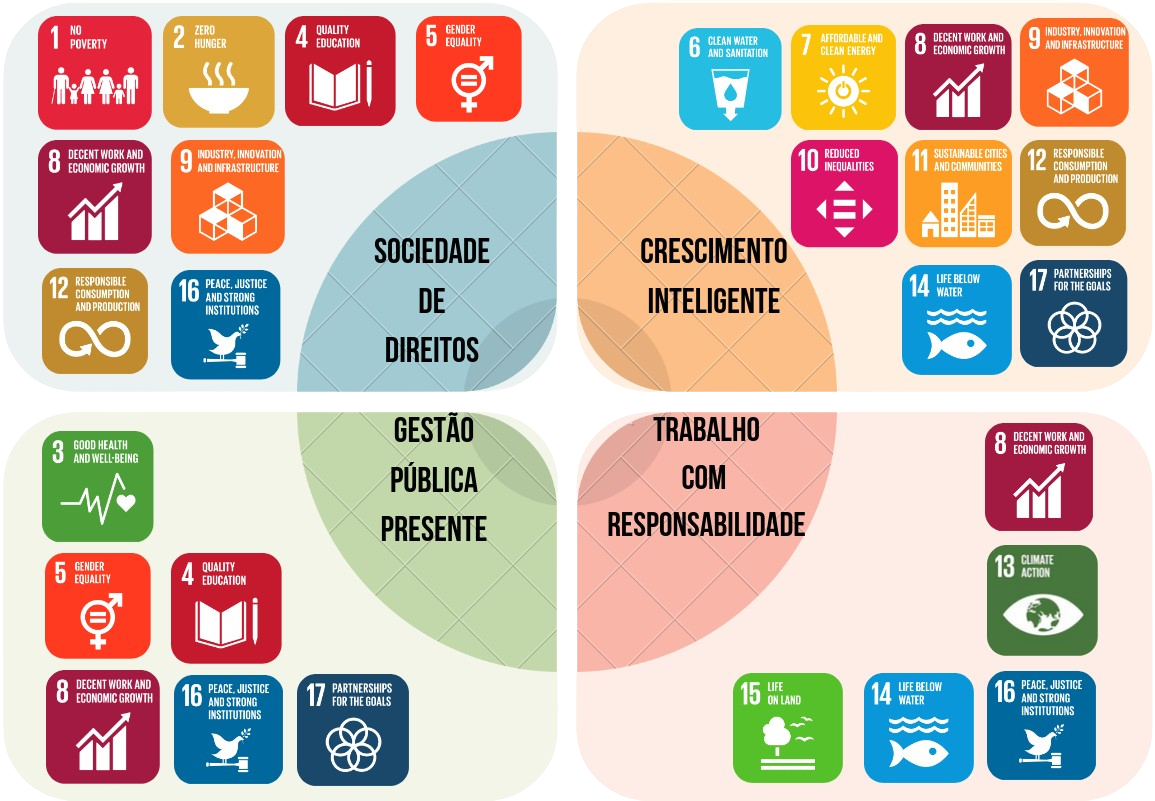
\includegraphics[width=.8\textwidth]{images/Figura.png}
        \caption{Eixos}
        \label{fig:ods}
    \end{figure}
\end{frame}

\section{Desenvolvimento}

\begin{frame}
    \frametitle{Slide 3}
    
     \begin{itemize}[<+->]
        \item Tópico 1
        \item Tópico 2
        \item Tópico 3
    \end{itemize}    
\end{frame}


\begin{frame}
    \frametitle{Slide 4}
        
     \begin{itemize}[<+->]
        \item Itens:
        \begin{itemize}
            \item Subitens:
            \begin{itemize}[<+->]
                \item Tópico 1; 
                \item Tópico 2;
                \item Tópico 3;
            \end{itemize} 
            \item Tópico X
        \end{itemize}
        \item Equação \ref{eq:equacao1}:
        \item[] \begin{equation} \label{eq:equacao1}
BSx =  \left\{ \left[ \dfrac{( DM_a - DM_x ) \times ( BS_a - BS_p )}{( DM_a - DM_p )} \right] (-1) \right\} + BS_a
\end{equation}
    \end{itemize}    
\end{frame} 


\section{Resultados}

\begin{frame}
    \frametitle{Slide 5}
    
    \begin{table}
    \centering
    \caption{Resumo dos artigos incluídos e principais indicadores de sustentabilidade}
    \label{tab:resumoIndicadores}
    \scriptsize
	\begin{tabular}{cll}
		\toprule
		\textbf{\#} & \textbf{Artigo} & \textbf{Indicador}  \\
		\midrule
		\textit{1} & \citeonline{MeloFariasKato2016} & \textit{MESMIS (MASERA et al, 1999)} \\
		\textit{2} & \citeonline{resque2017sustentabilidade} & \textit{MESMIS (MASERA et al, 1999)} \\
    	\textit{3} & \citeonline{Silva2016} & \textit{Barômetro da Sustentabilidade (PRESCOTT-ALLEN, 1995)} \\
		\textit{4} & \citeonline{Cardoso2016} & \textit{Barômetro da Sustentabilidade (PRESCOTT-ALLEN, 1995)} \\
		\textit{5} & \citeonline{Crispim2020} &
		  \begin{tabular}[c]{@{}l@{}}
    		{\textit{Barômetro da Sustentabilidade (PRESCOTT-ALLEN, 1995)}}\\
        	\textit{Índice de Desenv. Sust. para Municípios (IDSM)}\\
        	\textit{Índice de Desenv. Sust. para Municípios Part. (IDSMP)}\\
    	\end{tabular} \\
		\textit{6} & \citeonline{Vale2020} & \textit{Barômetro da Sustentabilidade (PRESCOTT-ALLEN, 1995)} \\
		\textit{7} & \citeonline{de2019diagnostico}  &
		  \begin{tabular}[c]{@{}l@{}}
		  \textit{Matriz de Indic. de Sust. p/ a GRSU}\\ (SANTIAGO E DIAS, 2012) 
		\end{tabular} \\
		\textit{8} & \citeonline{Cardoso2014}  & \textit{Barômetro da Sustentabilidade (PRESCOTT-ALLEN, 1995)} \\
		\textit{9} & \citeonline{Ferreira2018}  & \textit{Barômetro da Sustentabilidade (PRESCOTT-ALLEN, 1995)} \\
        \textit{10} & \cite{Camacho2021}  & \textit{Barômetro da Sustentabilidade (PRESCOTT-ALLEN, 1995)} \\
        \bottomrule
	\end{tabular}\\
     \centering{\footnotesize Fonte: Elaborado pelo autor.}
    \end{table}
    
\end{frame}

\begin{frame}
    \frametitle{Slide 6}
    
    \begin{table}
	\centering
	\caption{Quantidade de municípios por mesorregião}
	\label{quadro:tabela1}
    \scriptsize
	 \begin{tabular}{lcc}
		\toprule
		\textbf{Mesorregião} & \textbf{Quantidade de municípios}\\
		\midrule
		Baixo Amazonas & 14 \\
		Marajó & 16\\
    	Metropolitana de Belém & 11\\
		Nordeste Paraense & 49\\
		Sudeste Paraense & 39\\
		Sudoeste Paraense & 14\\
		\textbf{Total}  & \textbf{144}\\
		\bottomrule
	\end{tabular}\\
	{\footnotesize Fonte: Elaborado pelo autor. }
\end{table}
\end{frame} 

\section{Conclusão}


\begin{frame}
    \frametitle{Conclusões}
    \justifying
     \begin{itemize}[<+->]
        \item Tópico 1.
        \item Tópico 2.
        \item Tópico 3;
        \item Tópico 4.
     \end{itemize}
\end{frame} 


\section{Referências}

\begin{frame}[allowframebreaks]{Referências}
\bibliography{references}
\end{frame}

\begin{frame}
    \frametitle{Fim}
    \centering \huge Agradecimentos
    \vskip60px
    \begin{figure}
        \centering
        
\includegraphics[scale=.3]{otherResources/logo.png}
        
\includegraphics[scale=.3]{otherResources/ufpa.png}
    \end{figure}
\end{frame} 
%
%
\end{document}

